\eko{} has been compared with the benchmark tables
given in \cite{Giele:2002hx,Dittmar:2005ed}.
We find a good match except for a list of typos which we list here:
\begin{itemize}
    \item in table head in \cite{Giele:2002hx} should be $2xL_+ = 2x(\bar u + \bar d)$
    \item in the head of table 1: the value for $\alpha_s$ in \ffns{} is wrong (as pointed out and corrected in \cite{Dittmar:2005ed})
    \item in table 3, part 3 of \cite{Giele:2002hx}: $xL_-(x=10^{-4}, \muF^2 = \SI{1e4}{\GeV^2})=1.0121\cdot 10^{-4}$ (wrong exponent) and
          $xL_-(x=0.1, \mu_F^2 = \SI{1e4}{\GeV^2})=9.8435\cdot 10^{-3}$ (wrong exponent)
    \item in table 15, part 1 of \cite{Dittmar:2005ed}: $xd_v(x=10^{-4}, \mu_F^2 = \SI{1e4}{\GeV^2}) = 1.0699\cdot 10^{-4}$ (wrong exponent) and
          $xg(x=10^{-4}, \mu_F^2 = \SI{1e4}{\GeV^2}) = 9.9694\cdot 10^{2}$ (wrong exponent)
\end{itemize}
Some of these typos have been already reported in \cite{Diehl:2021gvs}.

\begin{figure}
    \centering
    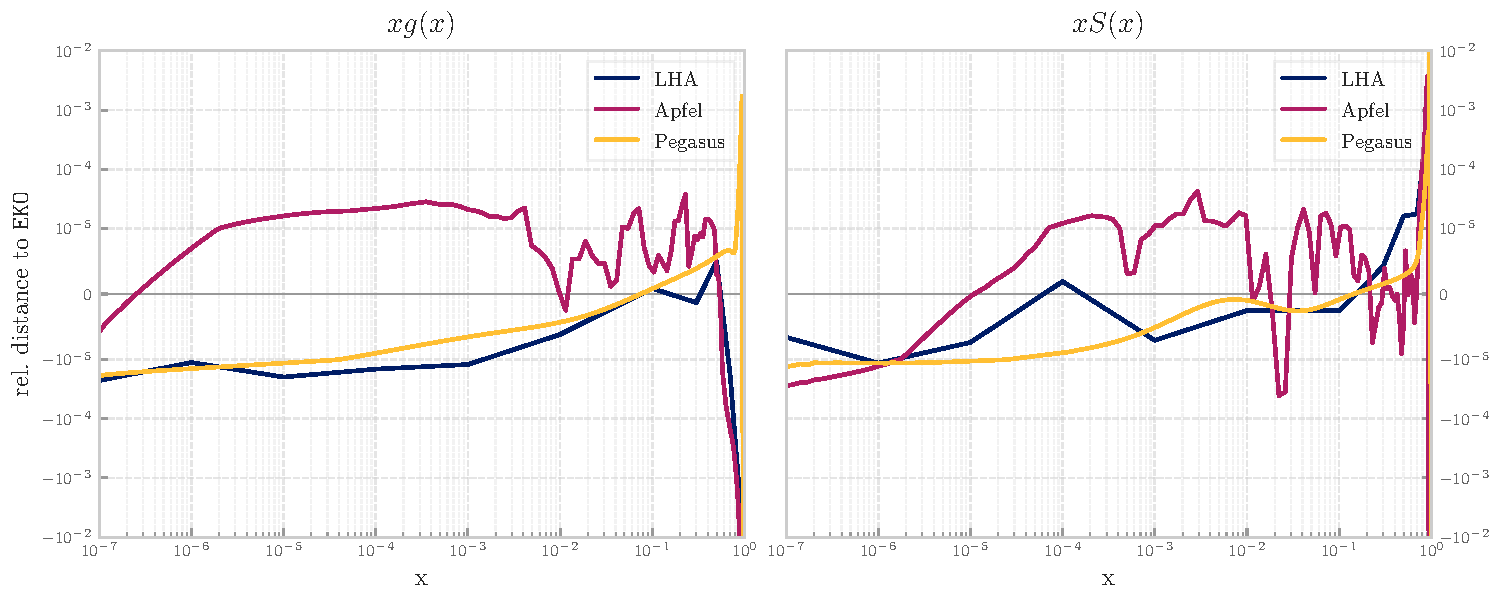
\includegraphics[width=\textwidth,height=.24\textheight]{ch-eko/lha_bench_g_S}
    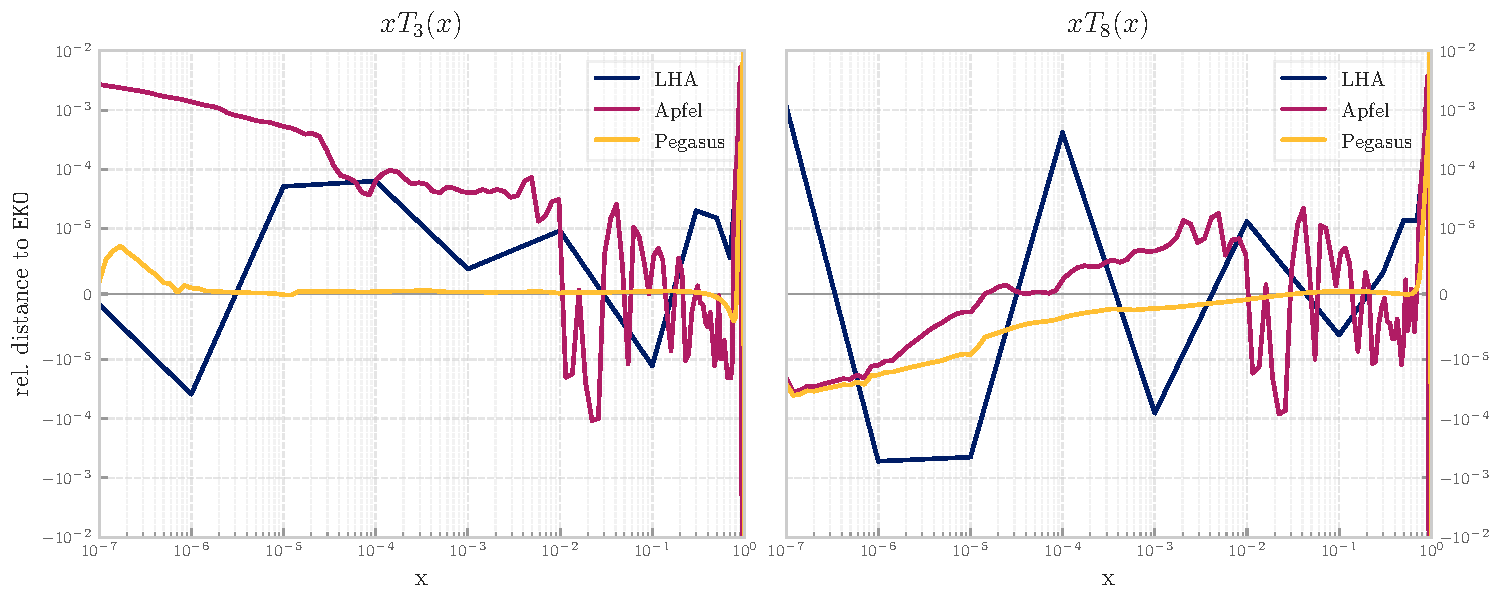
\includegraphics[width=\textwidth,height=.24\textheight]{ch-eko/lha_bench_T3_T8}
    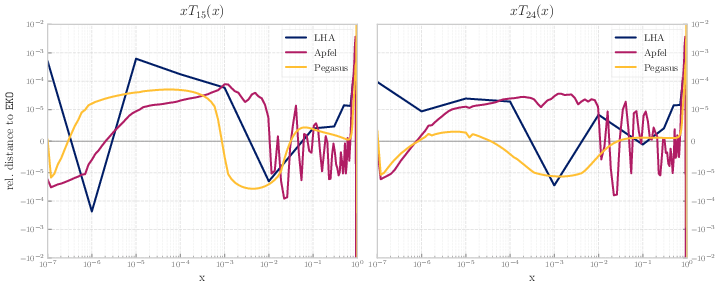
\includegraphics[width=\textwidth,height=.24\textheight]{ch-eko/lha_bench_T15_T24}
    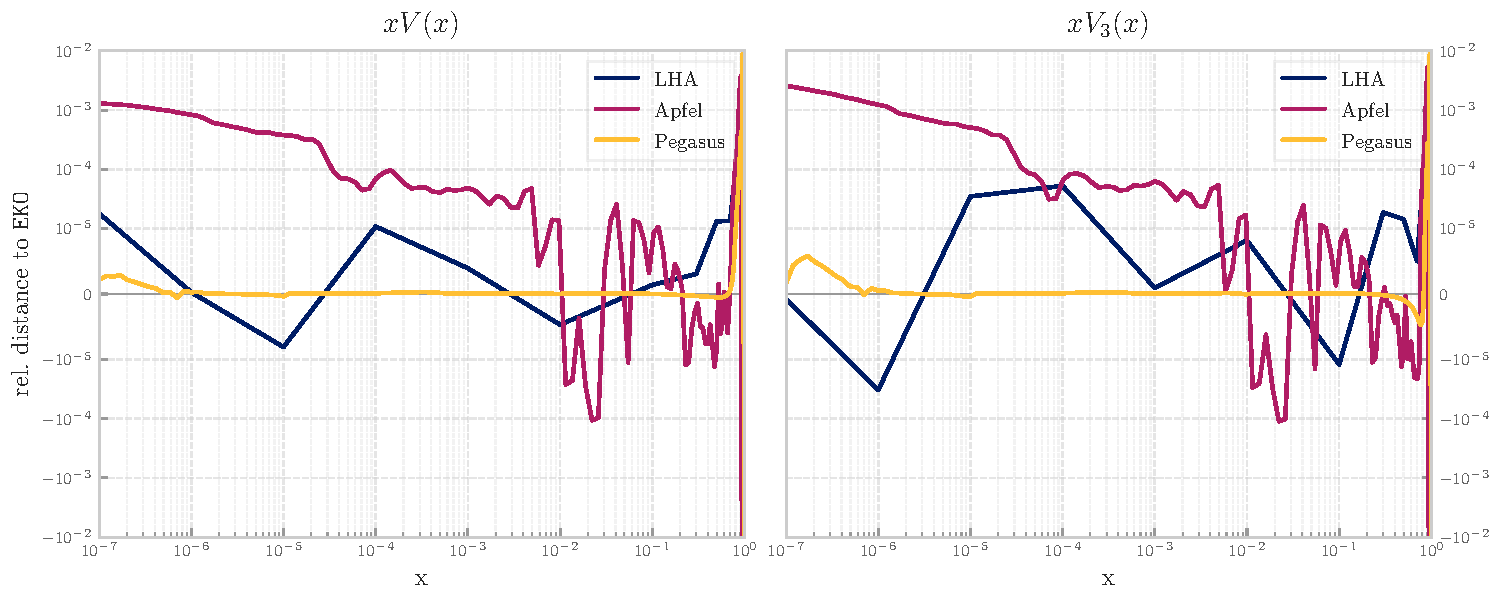
\includegraphics[width=\textwidth,height=.24\textheight]{ch-eko/lha_bench_V_V3}
    \caption{Relative differences between 
        the outcome of \nnlo{} \qcd{} evolution
        as implemented in \eko{} and the
        corresponding results from \cite{Dittmar:2005ed}, \apfel{}~\cite{Bertone:2013vaa} and \pegasus{}~\cite{Vogt:2004ns}.
        We adopt the settings of the Les Houches \pdf{} evolution benchmarks~\cite{Giele:2002hx,Dittmar:2005ed}.}
    \label{fig:LHAbench}
\end{figure}

In \cref{fig:LHAbench} we present the results of the \vfns{} benchmark at \nnlo{}, where a
toy \pdf{} is evolved from $\mu_{F,0}^2=\SI{2}{\GeV^2}$ up to $\mu_{F}^2=\SI{1e4}{\GeV^2}$
with equal values of the factorization and renormalization scales $\muF=\muR$.
For completeness, we display the singlet $S(x)$ and gluon $g(x)$ distribution (top), the singlet-like $T_{3,8,15,24}(x)$ (middle)
and the valence $V(x)$, valence-like $V_{3}(x)$ (bottom) along with
the results from \apfel{} and \pegasus{}. We find an overall agreement at the level of $O(10^{-3})$.
